\chapter{Implementation and Integration on Robots}
\label{chapt|implementation-integration}

\section{A centralised server-based implementation}
\label{sect|oro-server-impl}

The ORO server is a multi-platform command-line application that starts a
socket server to which clients can send requests to store or retrieve symbolic
statements.

Figure~\ref{fig|oro-impl} gives an overview of the ORO server architecture. The
server is build on three layers: a front-end, in charge of the communication
with external clients, a set of central modules that either handle incoming
requests or provide background processing (like the event monitoring or the
memory management), and a back-end, that stores the knowledge models in several
parallel pools of RDF triples, one per agent. The back-end provides all the
knowledge manipulation features required by the modules including
reasoning.

\begin{figure}
    \centering
    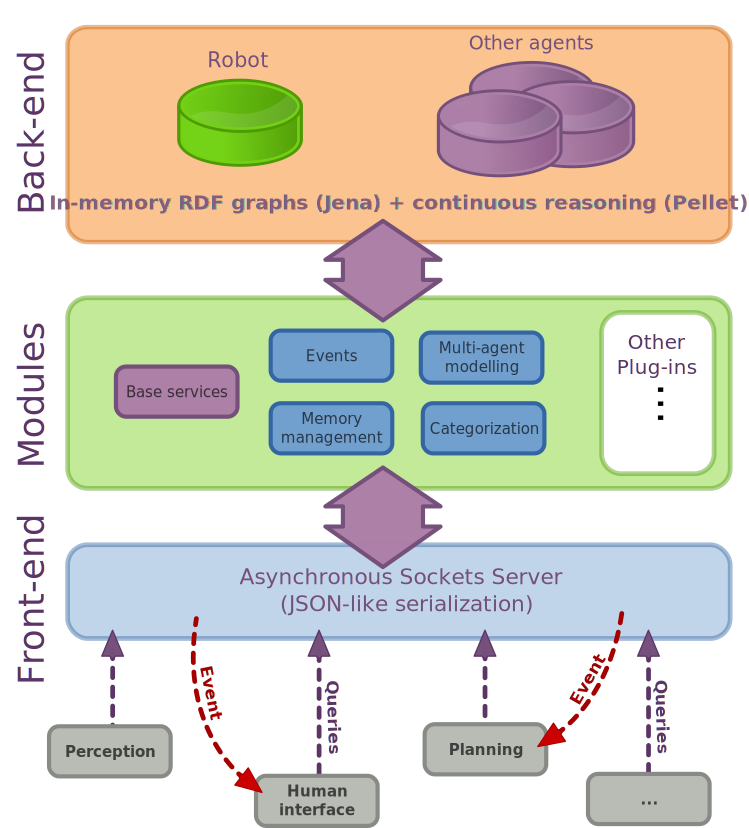
\includegraphics[width=0.7\columnwidth]{implementation/oro_impl.pdf}
    \caption{The software architecture of the ORO server.}
    \label{fig|oro-impl}
\end{figure}


The ORO server is written in Java 6. This choice is due to widespread use of
the Java language in the semantic Web community that leads to the fact that
most of the RDF/OWL API and reasoners are available as Java libraries. As
mentioned previously, the ORO server relies on the Open Jena API for OWL
manipulation and on the Pellet reasoner for all reasoning tasks. Java was thus
the best candidate to glue them in a robotic-friendly knowledge base.

\subsection{Front-end}
\label{sect|frontend}

Communication with external components is handled by the server front-end.  It
was originally build as a YARP node, but was eventually transformed into a
simpler and more generic socket interface.  The socket connector uses a simple
ASCII protocol, presented in figure~\ref{fig|oro-protocol}.  Communication with
dedicated robotic middlewares like ROS or YARP is provided by dedicated
external clients. Section~\ref{sect|interfacing-middlewares} briefly presents
them.

\begin{figure}
\centering
\footnotesize
\subtable[Client requests]{
    \begin{tabular}{p{3cm}|p{3cm}|p{3cm}}
    & {\tt \emph{method name}
    \emph{[parameter 1]}
    \emph{[parameter 2]}
    \emph{[parameter n]}
    \#end\#} & \\
    \end{tabular}
} \\
\subtable[Server answers]{
    \begin{tabular}{|p{3.5cm}|p{5cm}|p{2.5cm}|}
    {\tt ok \par
    \emph{[return value]}
    \#end\#} &
    {\tt error \par
    \emph{[exception name]}
    \emph{[human-readable error]}
    \#end\#} &
    {\tt event \par
    \emph{event id}
    \#end\#} \\
    \end{tabular}
}

\caption{The ORO server protocol. Elements in square brackets are optional.
Note that the {\tt ok} and {\tt error} message are synchronous server answers
to client requests while the {\tt event} message is produced asynchronously.}

\label{fig|oro-protocol}

\end{figure}


When a request is received by the front-end, it is parsed, deserialised and
dispatched to the module providing the requested service.

\subsection{Modules}

These \emph{modules} are initialised and maintained by the server. They provide
the actual features of the server as sets of \emph{services} (like \jmeth{add},
\jmeth{getSubclasses}, etc.).

Some modules do not expose any services. They provide instead other form of
knowledge management. For instance, the \jclass{MemoryModule} is in charge of
the application of the memory policies. It discards old statements depending on
the memory class they belong to (short term memory, long term memory, etc.).

Regular services (\ie that are actual Java methods) are invoked by the
front-end.  They process the request and interact with the knowledge pool via
the back-end interface.

\paragraph{Plugins} The server can be easily extended by the mean of
\emph{plugins}. These are JAR files that are loaded at run-time and have access
to the exact same internal APIs as regular modules like the event module or the
categorisation module. ORO comes with a tool that ease the creation of new
plugins by generating customisable templates. The process is documented in a
tutorial available
on-line\footnote{\url{http://www.openrobots.org/wiki/oro-server-plugins}}.

\subsection{Back-end}
\label{sect|backend}

The back-end consists in a pair \emph{\{triples store, reasoner\}}. For ORO,
we make the choice to rely the open-source {\sc Open Jena} library to store and
access the RDF graph, in combination with the {\sc Pellet} reasoner. However,
due to clean separation, other APIs (like the {\sc Manchester OWL-API}) and
reasoners (like {\sc Fact++} or {\sc HermiT}) could be used with little changes
in the back-end API.

\subsubsection{Open Jena}
\label{sect|jena}

{\sc Jena}~\cite{McBride2002} is a mature library for the semantic Web,
originally developed by Hewlett-Packard labs, and now under the leadership of
the Apache foundation.

As stated on its official website\footnote{{\sc Jena} website:
\url{http://incubator.apache.org/jena/}}, the Jena Framework includes:

\begin{itemize}
    \item an API for reading, processing and writing RDF data in XML, N-triples
    and Turtle formats;
    \item an ontology API for handling OWL and RDFS ontologies;
    \item its own rule-based inference engine for reasoning with RDF and OWL data
    sources;
    \item stores to allow large numbers of RDF triples to be efficiently stored
    on disk;
    \item a query engine compliant with the SPARQL specification
    \item servers to allow RDF data to be published to other applications using
    a variety of protocols, including SPARQL.
\end{itemize}

\subsubsection{Pellet}
\label{sect|pellet}

{\sc Pellet}~\cite{Sirin2007} is a reasoner for Description Logics developed by
Clark\&Parsia\footnote{{\sc Pellet} website:
\url{http://clarkparsia.com/pellet}}.

Pellet supports reasoning with the full expressiveness of OWL-DL
($\mathcal{SHOIN(D)}$) and OWL 2 ($\mathcal{SROIQ(D)}$).

Pellet provides all the standard inference services that are traditionally
provided by DL reasoners: consistency checking, concept satisfiability,
classification (computation of all the classes the instances belong to) and
realisation (the most specific classes that a specific individual belongs to).
It also supports DL-safe SWRL rule.

The use of a reasoner is completely transparent for the modules: the reasoner
is automatically called when a model changes to classify it. Thus, queries
to the knowledge models always access both the \emph{asserted} and
\emph{inferred} sets of statements. As a consequence, the ORO server can be run
with no reasoner without any visible API change for the modules. They will
simply manipulate only asserted facts.

\subsection{API}

As of version 0.8, the ORO server API exposes about 50 methods (some of them
are besides polymorphic) organised into seven categories: \emph{Base},
\emph{Agents}, \emph{Administration}, \emph{Concept comparison}, \emph{Events},
\emph{Queries} and \emph{Taxonomy walking}.

Partial support for the \emph{Knowledge API} (section~\ref{sect|knowledge-api})
has also been added to ORO server 0.8: the newly introduced {\tt revise} method
that takes a \emph{revision policy} as parameter is a versatile and generic
mechanism that deprecates {\it de-facto} several methods currently exposed by
the API.

The details of the current API is provided in appendix~\ref{chapt|oro-api}.

\subsection{Notes on the Java implementation}
\label{sect|java-impl}

The ORO server has been developed with modularity in mind, thus most of its
structure relies on clearly defined Java interfaces.
Figure~\ref{fig|oro-impl-java} presents the main ones.

\begin{figure}
    \centering
    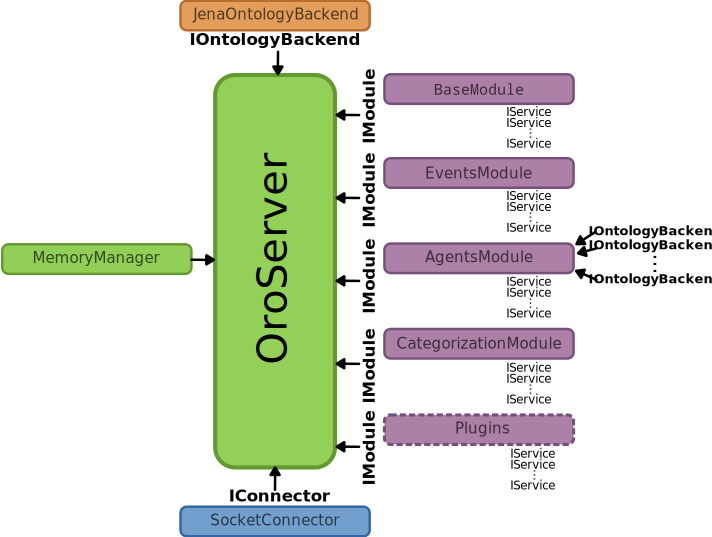
\includegraphics[width=0.9\columnwidth]{implementation/oro_impl_java.pdf}
    \caption{Main Java interfaces and classes of the ORO server.}
    \label{fig|oro-impl-java}
\end{figure}

The application entry point is the \jclass{OroServer} class. The class
instantiate one front-end (\jinterface{IConnector}), one main back-end
(\jinterface{IOntologyBackend}) and several modules (\jinterface{IModule}),
including plugins that are loaded at run-time.

Modules usually also implement the \jinterface{IServiceProvider} interface to
expose \emph{services} (\jinterface{IService}). These are the actual methods
found in the server API. Java methods that belongs to the API simply need to be
decorated with a \jinterface{@RPCMethod} Java annotation to be automatically
exposed. Extending the server API is thus simply a matter of annotating almost
any Java method\footnote{The only constraint being the input and output
datatypes: currently, primitive types, simple collections and objects with
explicit serialisation/deserialisation methods are supported.} with
\jinterface{@RPCMethod}. Listing~\ref{code|oro-add} shows one example of a
service annotated in such a way, the {\tt add} method. This method convert a
set of strings representing triples into \jinterface{IStatements}, and add them
to the triple store with the back-end method \jmeth{oro.add}.

\lstset{language=java}
\begin{lstlisting}[caption=The {\tt add} method from ORO {\tt BaseModule}, 
                   label = code|oro-add, 
                   morekeywords={@RPCMethod}]
@RPCMethod(
        category="base",
        desc="adds one or several statements (triples S-P-O)."
)
public void add(Set<String> rawStmts, String memProfile)
{
    Set<IStatement> stmtsToAdd = new HashSet<IStatement>();
    
    for (String rawStmt : rawStmts) {
        if (rawStmt == null)
            throw new IllegalStatementException("Got a null stmt!");
        IStatement s = oro.createStatement(rawStmt);
        stmtsToAdd.add(s);
    }
    
    oro.add(stmtsToAdd, MemoryProfile.fromString(memProfile), false);
}
\end{lstlisting}

As visible on the figure~\ref{fig|oro-impl-java}, the \jclass{AgentsModule}
plays a particular role: it manages the alternative knowledge models of other
agents, and store a \jinterface{IOntologyBackend} for each of them. This module
also re-export a large part of the services exposed by the \jclass{BaseModule}
(methods for standard knowledge manipulation), but in their multi-agent
versions.

This design issue (duplication of certain basic services) is due to the
historical development of the ORO server, and should be improved in future
versions.

%%%%%%%%%%%%%%%%%
\section{Bindings to other languages and components}
\label{sect|interfacing}

To ensure the integration of the ORO server in existing robotic architectures, we
have developed several idiomatic language-specific bindings, as well as bridges
with two widespread robotic middlewares, ROS and YARP.

\subsection{Language bindings}
\label{sect|bindings}

The main interaction gate with the ORO server is its socket interface (as
presented above, at section~\ref{sect|frontend}). Sockets are light-weight,
platform independent, and supported by every programming languages.  Developing
an interface with ORO server in a new language is hence relatively easy.

For our own needs, and because they are amongst the most widely used languages,
bindings for Python and C++ are available by default with ORO server.

The complete Python and C++ API will not be presented here (their
documentations are available
on-line\footnote{\url{http://www.openrobots.org/wiki/oro-server-bindings}}),
but we present two short example that demonstrate how the knowledge base can be
integrated in code in a natural way.

\subsubsection{Python}
\label{sect|python-bindings}

The Python script below (listing~\ref{code|ex-python}) demonstrates several of
the interaction mechanisms with ORO server: model alteration, queries and events.

\lstset{language=python}
\begin{lstlisting}[numbers=left,
                   caption=Example of interaction with {\tt oro-server} in Python, 
                   label = code|ex-python,
                   morekeywords={as}]
import time
import pyoro

def onEvent(evt):
        print("God save the queen! " + evt + " killed Bond!")

try:
        oro = pyoro.Oro()

        oro += ["Spy rdfs:subClassOf Human", 
                "bond rdf:type Spy", 
                "bond rdfs:label \"Bond, James Bond\""]

        if "bond rdf:type Human" in oro:
            print("Alright, Bond is a human")

        oro += "pr2 rdf:type Robot"

        for ag in oro["* rdf:type Agent"]:
            print("Agent " + ag + " is here.")

        oro.subscribe(["?a kills bond"], onEvent)
        oro += "pr2 kills bond"

        time.sleep(1)
        # the event should have been triggered

except pyoro.OroServerError as ose:
        print('Oups! An error occured!')
        print(ose)

finally:
        oro.close()
\end{lstlisting}

At line 8, we establish the connection to the server. We assume here that the
server is launched on the default port and on the local machine.

At line 10, three facts are added to the knowledge base. The first one modifies
the TBox of the ontology (alteration of the knowledge structure) while the two
other ones modify the ABox (a new instance and a new label). Adding (or
removing) triples from the ontology is done naturally with the {\tt +=} and
{\tt -=} operators.

At line 14, we check that a fact holds, either in the asserted model or in the
inferred model (in this case, Bond is inferred to be a human because we added
before that spies are types of humans). Here as well we use a natural idiomatic
Python syntax that creates and executes a SPARQL query behind the scenes.

Line 19 shows another way to execute queries, with a dictionary-like accessor.
Both humans and robots are asserted to be agents in the ORO common-sense
ontology, thus this query returns a list {\tt [bond, pr2]}.

Line 22 shows how events are created. We first subscribe to an event by passing
a pattern ({\tt ?a kills bond}) and a callback (implemented at lines 4-5).
Line 23 triggers the event, and the callback method is then invoked.

We have kept this example simple. The complete Python API allows to describe
more complex events (when a fact can not be inferred, when a new instance of a
given class appears, etc.), to manipulate different models, to walk through the
ontology taxonomy, etc.

\subsubsection{C++}

The C++ bindings are provided as a library called {\tt liboro}. The
listing~\ref{code|ex-cpp} presents some examples of its usage.

\lstset{language=c++}
\begin{lstlisting}[numbers=left,caption=Example of interaction with {\tt oro-server} in C++, label = code|ex-cpp]
#include <iostream>
#include <iterator>
#include <set>

#include "liboro/oro.h"
#include "liboro/oro_library.h" // static library of ORO concepts
#include "liboro/socket_connector.h"

using namespace std;
using namespace oro;

class EventCallback : public OroEventObserver {
    void operator()(const OroEvent& evt) {
        cout << "Event triggered!" << endl;
    }
};
  
int main(void) {
  set<string> partial_stmts;
  set<Concept> result;
  
  SocketConnector connector("localhost", "6969");
  Ontology *oro = Ontology::createWithConnector(connector);
  
  //Creation of instances
  Agent robot1 = Agent::create("Nice Robot", Classes::Robot);
  Agent human = Agent::create("Young PhD", Classes::Human);
  
  //First query
  partial_stmts.insert("?mysterious rdf:type Agent");
  oro->find("mysterious", partial_stmts, result);
  
  copy(result.begin(), 
       result.end(), 
       ostream_iterator<Concept>(cout, "\n"));
  
  partial_stmts.clear();
  result.clear();
  
  //More statements are added to the knowledge base
  Object table = Object::create(Classes::Table);

  Object unknown_object = Object::create();
  unknown_object.assertThat(Properties::isOn, table);
  
  oro->add(Statement("oro:isOn rdfs:subClassOf oro:isAt"));
  
  Agent myself("myself");
  
  myself.sees(unknown_object);
  myself.sees(human);
  
  //A query involving multiple partial statements
  partial_stmts.insert("?mysterious isAt ?support");
  partial_stmts.insert("?support rdf:type cyc:Table");
  partial_stmts.insert("myself sees ?mysterious");
  
  oro->find("mysterious", partial_stmts, result);
  
  copy(result.begin(), 
       result.end(), 
       ostream_iterator<Concept>(cout, "\n"));
  
  //Events
  EventCallback ec;
  Classes::Human.onNewInstance(ec);
  Agent superman = Agent::create("Superman", Classes::Human);
  
  sleep(1);
  
  set<string> event_pattern;
  Property flyingProp = Property("isFlying");
  
  event_pattern.insert( superman.id() + " isFlying true");
  oro->registerEvent(ec, 
                     FACT_CHECKING, 
                     ON_TRUE_ONE_SHOT, 
                     event_pattern, "");
  
  superman.assertThat(flyingProp, "true");
  
  sleep(1);
  
  return 0;
}

\end{lstlisting}

At lines 22 and 23, the {\tt oro} object is built as a singleton. This
actually connects the application to the ontology server.

At line 26 and 27, we create two new instances of agents labeled \emph{Nice
Robot} and \emph{Young PhD} (the static types {\tt Classes::Robot} and {\tt
Classes::Human} are generated from the ontology itself by a script).

A first simple query (line 30 and 31) return a {\tt std::set} of concept IDs.

At line 41, a new object is created. No label is defined, but the
class is set to be a table. On the contrary, at line 43, we create a generic
object (only asserting it is an instance of {\tt Object}).

At line 44, we assert a property (here also, the list of available properties is
statically generated from the ORO ontology).

As shown at line 46, we can as well access the ontology at a lower level,
directly adding (or removing) new triples. In this case, we modify the TBox of
the knowledge base.

C++ objects can also be created by using directly the concept IDs, as shown
line 48 for the special concept {\tt myself} (an instance always representing
the robot itself).

Some object properties frequently used in the ontology are
available as methods, as seen lines 50 and 51.

Lines 54 to 58 show a more complex query, involving several partial statements.
Named variables (like {\tt ?mysterious} or {\tt support}) are used in the
statements to reference the same entities.

Lastly, lines 65 to 80 show two ways of defining events with a callback functor
(defined at lines 12-16).

To deal with real-world constraints, {\tt liboro} also provides mechanisms to
reconnect to the ontology server when the connection is lost, and has a
built-in buffering system to increase bandwidth for components that produce a
large amount of symbolic facts.

\subsection{Interface with robotic middlewares}
\label{sect|interfacing-middlewares}

While convenient in certain cases, language-level interfaces do not usually
offer the modularity and loose-coupling required by complex robotic
architectures where tenth of modules, possibly spread over several computers,
need to talk together. The acknowledgement of this issue has led to the
development over the last ten years of numerous so-called \emph{robotic
middlewares} that abstract away inter-module communication (at the transports,
protocols and programming interfaces levels).

We provide with ORO server wrappers for two of the main middlewares currently
in use in the robotic community, ROS~\cite{Quigley2009} and
YARP~\cite{Metta2006}.

These wrappers use the C++ or Python bindings previously presented to expose
the features of ORO server as a stand-alone ROS/YARP nodes.

%%%%%%%%%%%%%%%%%
\section{Monitoring and debugging}
\label{sect|monitoring}

\subsection{Logging and debugging tools}

The ORO server offers several levels of logging, from almost silent to very
verbose. In verbose mode ({\tt debug} level), the server outputs exact incoming
requests, along with millisecond accurate timestamps.

Those logs can then be replayed by a special tool written in Python that
simulates the original communication with the server: timestamps are respected
and if multiple clients where connected to the server, the log player forks one
thread by client to simulate parallel access to the server.

Also available to the developer, an explanation of the inconsistencies when
they occur is produced by the server, and helps to retrace the sequence of
logical steps that led to the inconsistency.

\subsection{Visualisation}
\label{sect|oroview}

\begin{figure}
    \centering
    \subfigure{}{
        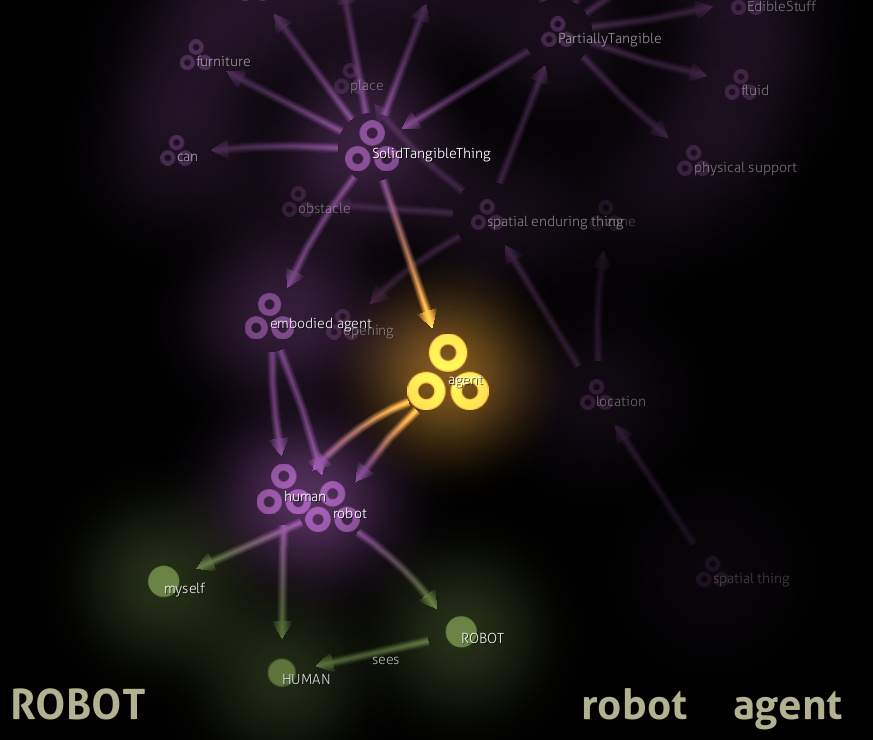
\includegraphics[width=0.41\columnwidth]{implementation/oroview.jpg}
        }
    \subfigure{}{
        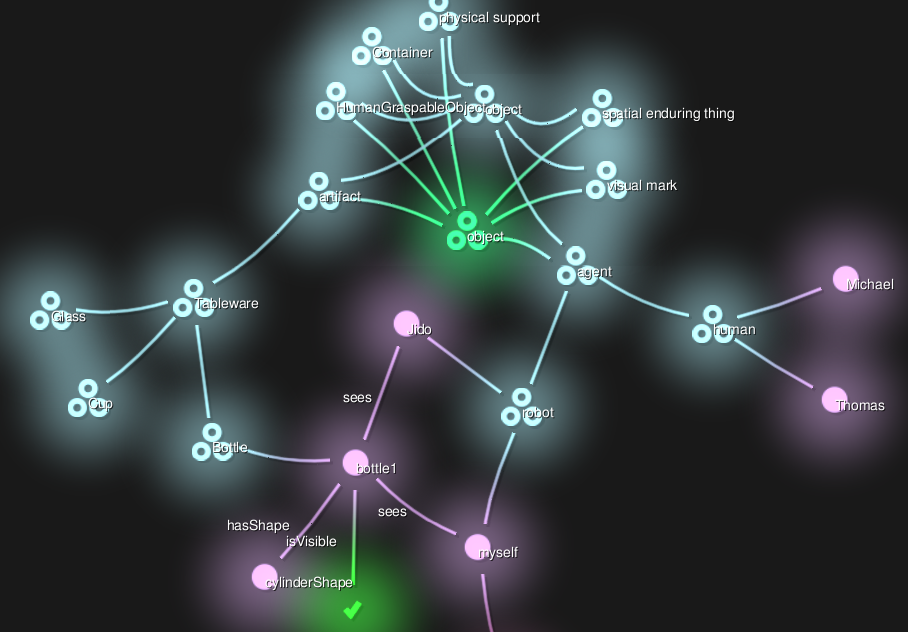
\includegraphics[width=0.5\columnwidth]{implementation/oroview2.png}
        }

    \caption{Two screenshots of the {\tt oro-view} visualisation tool. On the
    left one, an \concept{ActiveConcept} (in yellow) is visible.}

    \label{fig|oroview}
\end{figure}

Visualisation of ontologies is a difficult task in general because of their
complex graph structure. In order to present anyway the content of the ontology
to external observers, we have developed an OpenGL-based dynamic visualiser
called {\tt oro-view} (figure~\ref{fig|oroview}). This application connects to
the ORO server and lets the user explore the taxonomy by simply selecting
concepts on the screen. Nodes are then expanded, distributed in a force-directed
layout, and further reveal the structure of the ontology. Because {\tt oro-view}
takes on-demand its input from the server, changes in the ontology (new facts
being added, etc.) are reflected in the viewer when the user refreshes nodes.

{\tt oro-view} also subscribes at start-up to a special event for \emph{active
concepts} (it monitors new instances of the \concept{ActiveConcept} class).
Each time an individual is asserted to be an \concept{ActiveConcept}, the
server triggers back {\tt oro-view} that creates a visual focus on the concept
(the individual ``pops up''). When displayed during experiments, this provides
visual feedback to external observers. In particular, we made use
of this feedback during the public performance of the \emph{Roboscopie} theatre
play (section~\ref{sect|roboscopie}).

{\tt oro-view} also provides export to GraphViz {\tt dot} format for latter
reuse of the ontology graph in publications.

%%%%%%%%%%%%%%%%%
\section{Integration in the robot architecture}
\label{sect|integration}

\begin{figure*}[thpb]
  \centering
  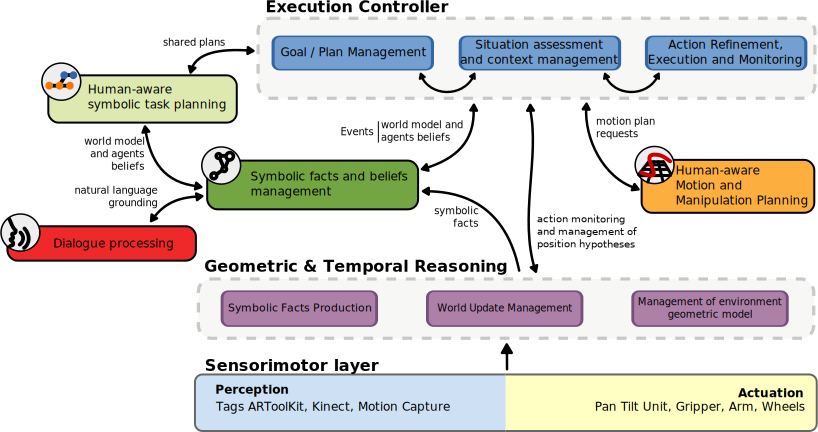
\includegraphics[width=\columnwidth]{integration/architecture_overview.pdf}

  \caption {Software architecture of PR2 and Jido, two service robot
  interacting with humans at LAAS-CNRS.}

  \label{fig|archi}
\end{figure*}

Figure~\ref{fig|archi} presents the organisation of the upper software layer
(the ``decisional'' or ``cognitive'' layer) of the service robots Jido and PR2
as currently in service at LAAS (this architecture is described in detail
in~\cite{Alami2011}). The sensori-motor layer (bottom) is abstracted in SPARK,
an intermediate amodal 3D model where geometric (and some temporal) reasoning
take place.

The outcome of the geometric analysis, as well as the result of the dialogue
processing module ({\sc Dialogs}), are stored in ORO, that plays the role of as
a central knowledge hub. The symbolic knowledge base triggers events that are
captured by a top-level execution controller.

In our architecture, the controller can rely on two specialised planners: MHP,
a geometric motion and manipulation planner~\cite{Sisbot2008, Mainprice2011,
Pandey2010} and HATP, a symbolic task planner~\cite{Alili2009}.

The dialogue processing module, as well as the symbolic task planner, also use
the knowledge base to answer questions or initialise the planning domain.

During a typical interaction experiment (such an experiment is describe at
chapter~\ref{chapt|evaluation}), the execution controller decides upon a goal
to reach, requires a plan from the task planner, allocates the actions to the
human and the robot, communicates the shared plan to the human, and controls
and monitors its execution. The operation continues until the goal is achieved,
is declared unachievable or is abandoned by the human.

In this architecture, only ORO and Dialogs (the dialogue processing module that
we present in the next chapter), as components, are the actual direct outcomes
of this doctoral work. It is however important to present the other one all
here as well since a knowledge base only make sense within a larger
architecture, with knowledge providers and consumers.  Furthermore, the
approach to knowledge management introduced by this thesis had a strong
influence on the design of the communication flows between all these
components. Thus, this section introduces the software components that have
been used in conjunction with ORO (mostly, but not only, on the LAAS robots),
and details how these components produce, exchange and consume symbolic
knowledge.

\subsection{Acquiring and anchoring knowledge in the physical world: the SPARK module}
\label{sect|spark}

Anchoring perceptions in a symbolic model requires perception abilities and
their symbolic interpretation. In this section we present SPARK (\emph{SPAtial
Reasoning \& Knowledge}~\cite{Sisbot2011}), a situation assessment reasoner
that generates symbolic knowledge from the geometry of the environment with
respect to relations between objects, robots and humans, also taking into
account the different perspective that each agent has on the environment.

SPARK can be seen as an amodal geometric model of the environment that serves
both as basis for the fusion of the perception modalities and as bridge with
the symbolic layer.

Figure~\ref{fig|spark} shows a screenshot of the SPARK environment side-by-side
with the real environment. In this example, objects are
identified and localised through 2D barcodes. The human pose is tracked with
a Kinect-like device (assisted by motion capture to accurately track the
head motion, which is required to compute what the human is looking at).

The geometric model is continuously updated at run-time by the robot.

\subsubsection{Building an agent-aware symbolic model of the environment}
\label{sect|situ}

\paragraph{On Perspective Taking} Visual perspective taking refers to the
ability for visually perceiving the environment from other's point of view.
This ability allows us to identify the objects in situations where the visual
perception of one person differs from the other one. In developmental
psychology, one typical example consists of two similar objects in a room (\eg.
two balls) where both are visible for the child, but only one is visible for
the adult. Thus, when the adult asks the child to hand over ``the ball'', the
child is able to correctly identify which ball the adult is referring to (\ie
the one visible from the adult point of view), without asking~\cite{Moll2006}.

Besides, in order to compute a visual perspective, the actual visibility alone
is not enough. We include not only what the other person sees in a given
moment, but also what he \emph{can} see with a minimal effort (moving the eyes
or the head). To model the potential visibility of an object we compute a
visibility ratio while turning the head of the agent model towards the object
(figure~\ref{fig::sparkRepresentations},
page~\pageref{fig::sparkRepresentations}).

Spatial perspective taking refers to the qualitative spatial location of
objects (or agents) with respect to a frame (\eg \emph{the keys on my left}).
Based on this frame of reference, the description of an object
varies~\cite{Marin2008}. Humans mix perspectives frequently during interaction.
This is more effective than maintaining a consistent one, either because the
(cognitive) cost of switching is lower than remaining with the same
perspective, or if the cost is about the same, because the spatial situation
may be more easily described from one perspective rather than
another~\cite{Tversky1999}. Ambiguities arise when one speaker refers to an
object within a reference system (or changes the reference system, \ie switches
perspective) without informing his/her partner about it~\cite{Breazeal2006,
Ros2010}. For example, the speaker could ask for the ``keys on the left''.
Since no reference system has been given, the listener would not know where
exactly to look.  However, asking for ``the keys on your left'' gives enough
information to the listener to understand where the speaker is referring to. On
the contrary, when using an exact, unambiguous term of reference to describe a
location (\eg. ``go north'') no ambiguity arises.

In this work, we use two types of the frames of reference: egocentric (from the
robot perspective) and addressee-centred (from the human perspective).

\begin{figure}[ht!]
   \begin{center}
%
       \subfigure{
           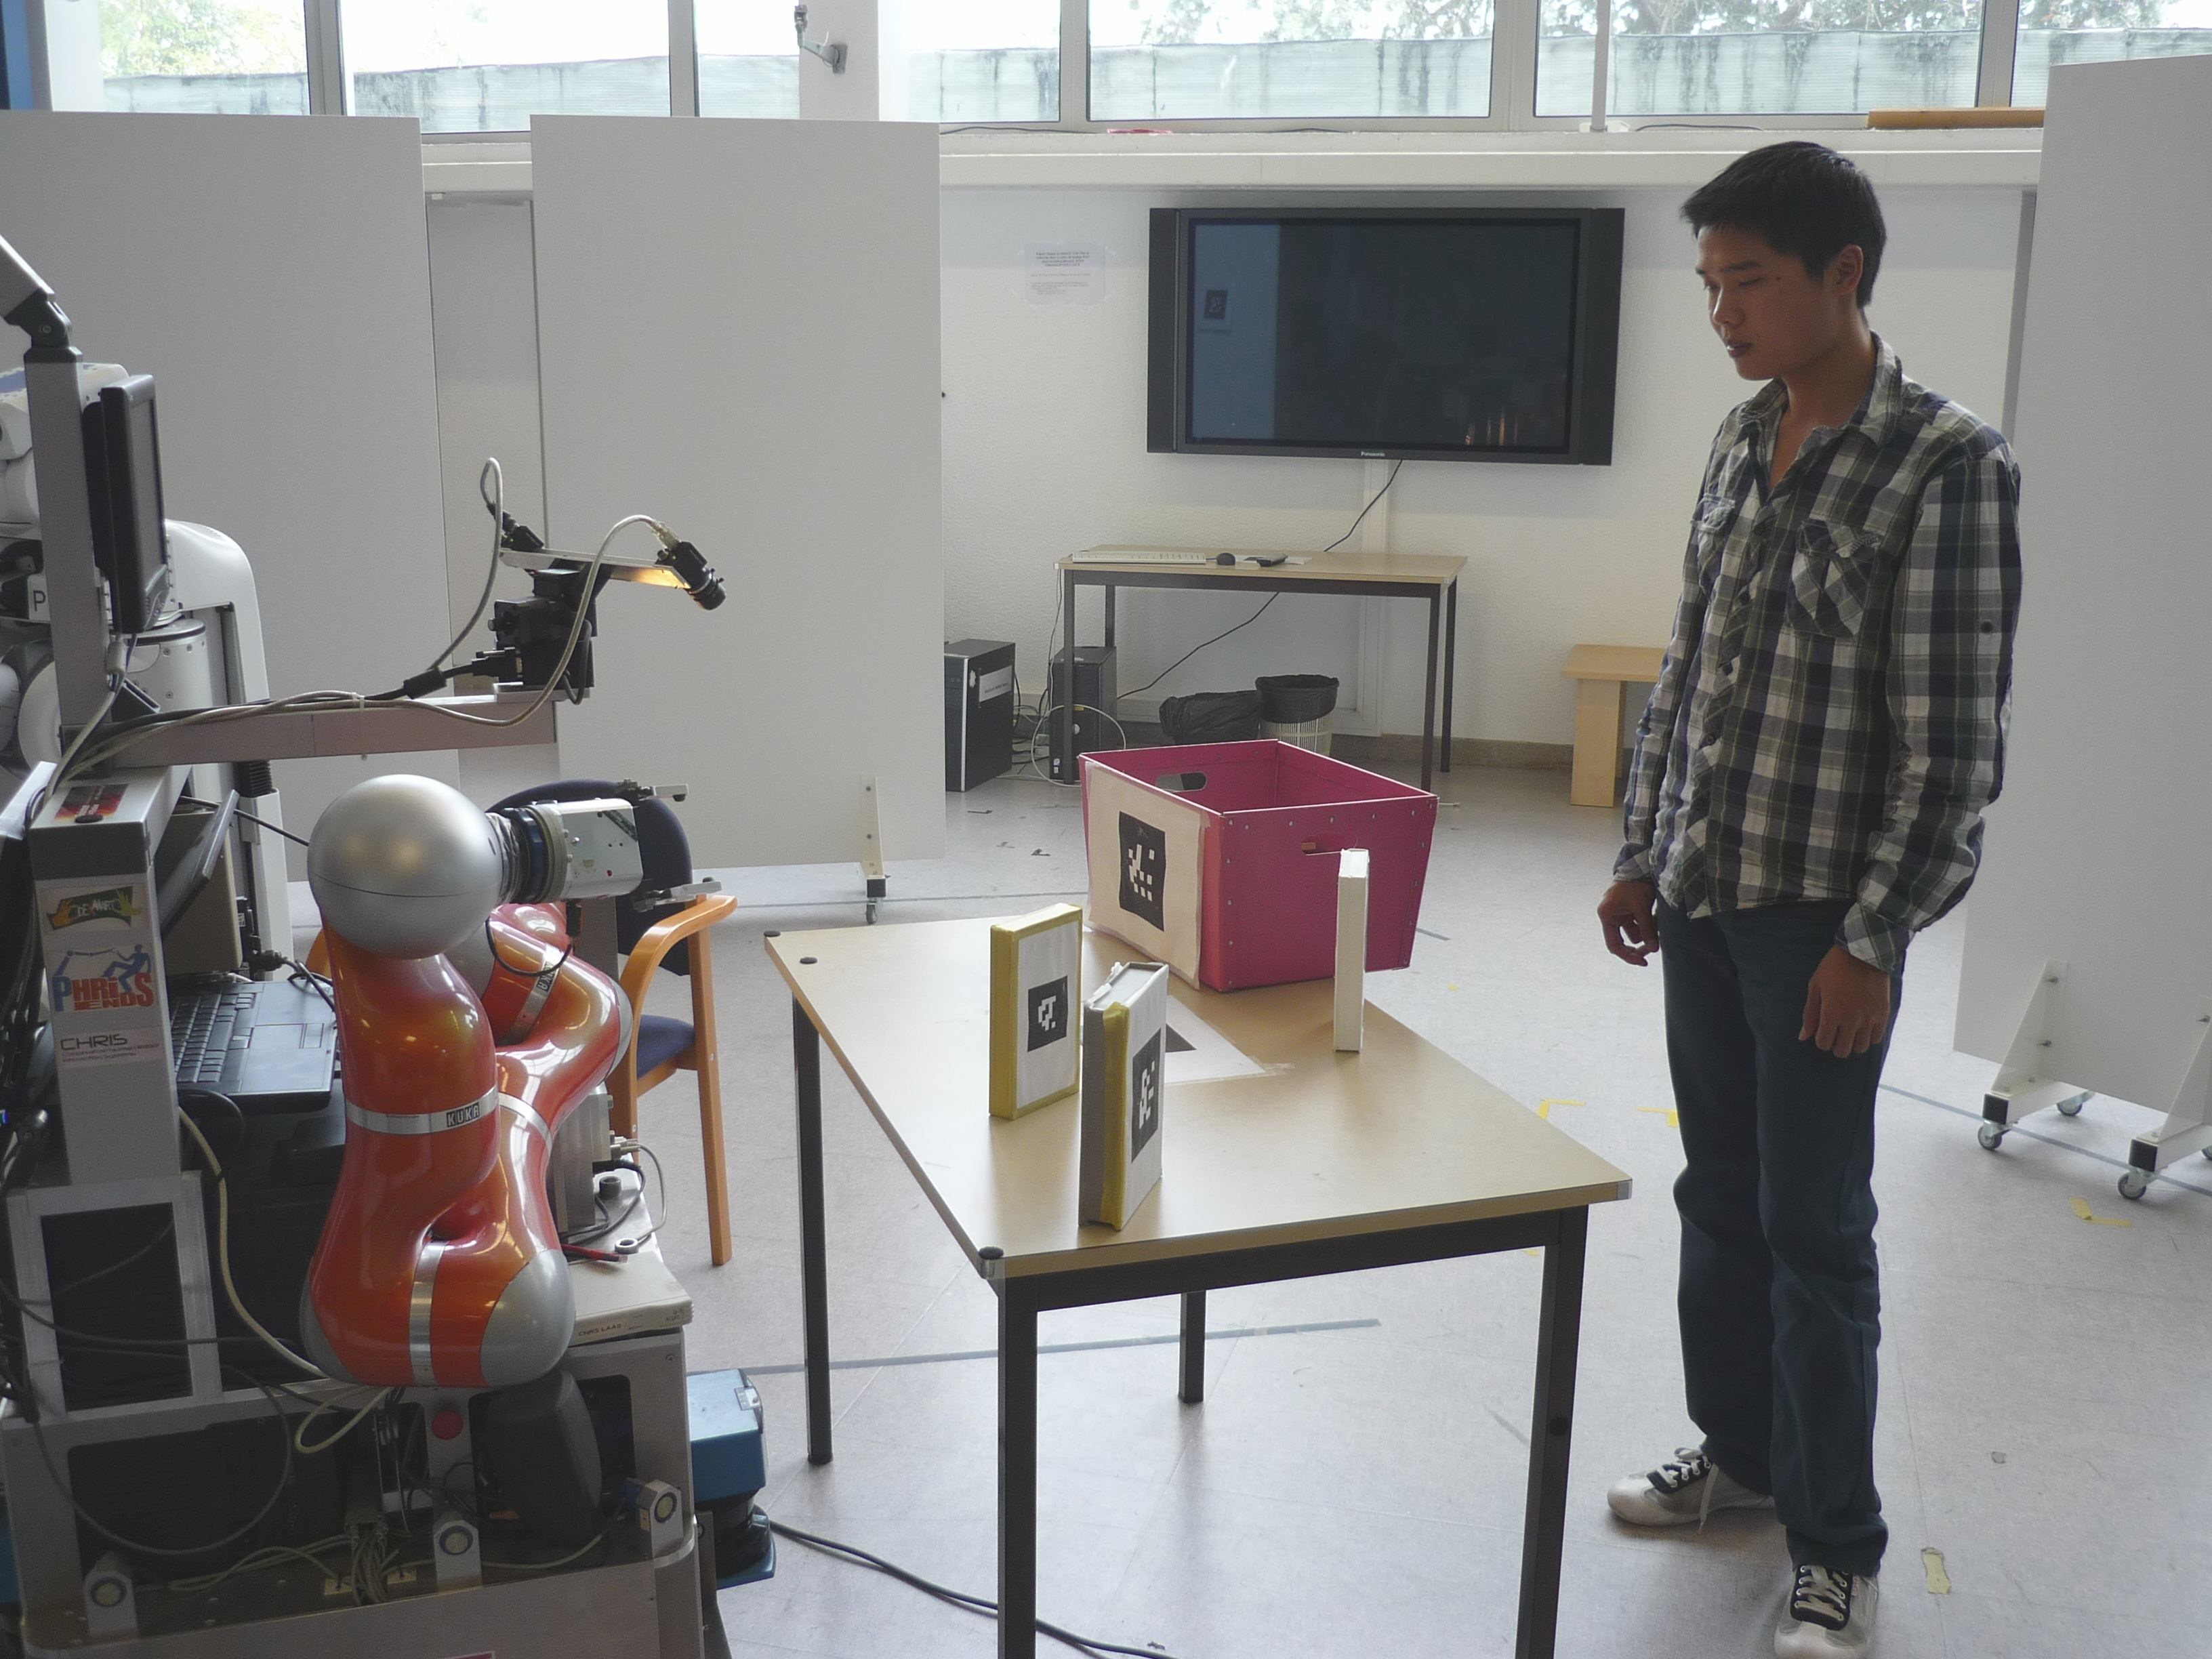
\includegraphics[width=0.5\textwidth]{spark/etat.jpg}
       }%
       \subfigure{%
          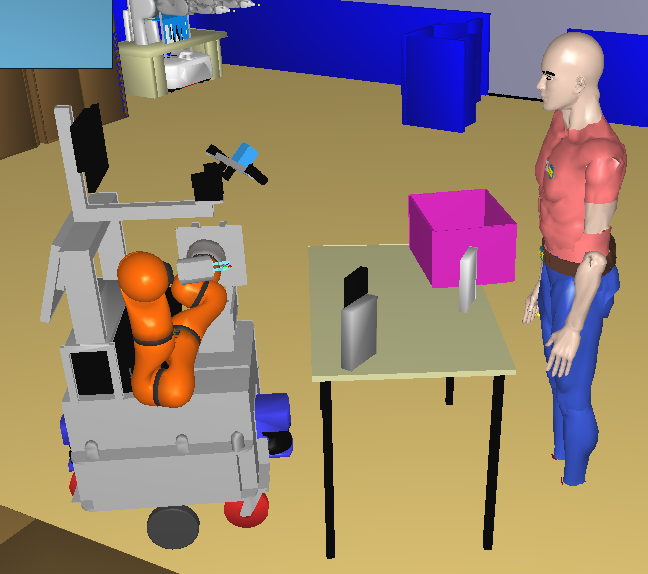
\includegraphics[width=0.43\textwidth]{spark/etat_spark.png}
       }\\ %  ------- End of the first row ----------------------%
%
   \end{center}

   \caption{The robot represents at run-time its environment in a 3D model
   resulting of the sensors' inputs fusion (Kinect, motion capture, 2D barcodes
   tracking).}

   \label{fig|spark}

\end{figure}

\paragraph{Symbolic locations}

Human commonly refer to the positions of objects with symbolic descriptors
(like \emph{on}, \emph{next to}...) instead of precise, absolute positions.
These type of descriptors have been studied in the context of language
grounding \cite{O'Keefe1999,Matuszek2010,Regier2001,Kelleher2006,Blisard2005}.
In SPARK we focus agent-independent symbolic locations and agent-dependent,
relative locations.

\paragraph{Agent-independent locations}

We can refer to object locations with respect to other objects in the
environment, such as \emph{above, next to, in}, etc. SPARK computes
three main relations based on the bounding box and centre of mass of the
objects (fig.~\ref{fig|sprelations}): 

\begin{itemize}
	\item \concept{isOn}: computes if an object $O_1$ is on another object $O_2$ by
	evaluating the center of mass of $O_1$ according to the bounding box of $O_2$.

	\item \concept{isIn}: evaluates if an object $O_1$ is inside another object
	$O_2$ based on their bounding boxes $BB_{O_1}$ and $BB_{O_2}$.

	\item \concept{isNextTo}: indicates whether an object $O_1$ is next to another
	object $O_2$. We cannot use a simple distance threshold to determine if two
	objects are next to each other since the relation is highly dependent on the
	dimensions of the objects. For instance, the maximum distance between large
	objects (\eg two houses) to consider them as being next to each other is much
	larger than the maximum distance we would consider for two small objects (\eg
	two bottles). Thus, the relation between the dimensions and the distances of
	the objects are taken into account.  

\begin{figure} 
	\centering
	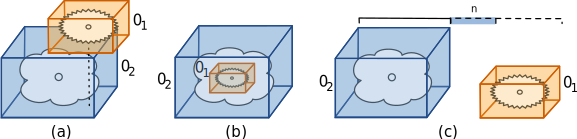
\includegraphics[width=0.95\columnwidth]{spark/spatial_relation.pdf}
	\caption{Spatial relations between two objects: (a) \concept{isOn} relation, 
	(b) \concept{isIn} relation, and (c) \concept{isNextTo} relation.} 
	\label{fig|sprelations} 
\end{figure}

\end{itemize} 

To ensure the different agent models are up-to-date, all these properties are
always computed on-line, each time the current state of the world changes.

Table~\ref{facts|sprelations} lists all the symbolic placement relationships
that are currently computed by the system.

\renewcommand{\concept}[1]{{\scriptsize \texttt{#1}}}
\begin{table}[h]
    \centering
    \begin{tabular}{p{1.5cm}lp{2cm}p{3.7cm}}
	\rowcolor{white}
    \textbf{Subject} & \textbf{Predicate} & \textbf{Object} & \emph{Notes} \\ 
    \hline
	 \concept{Location} & \concept{isAt} $\equiv$ \concept{cyc:objectFoundInLocation}  &  \concept{Location} & \\ 
	 &  $\rightarrow$ \concept{isOn} $\equiv$ \concept{cyc:above\_Touching}  &  & \\ 
	 &  $\rightarrow$ \concept{isIn}  &  & \\ 
	 &  $\rightarrow$ \concept{isNextTo}  & &  \\ 
	 \concept{Location}  & \concept{isAbove} $\equiv$ \concept{cyc:above-Generally}  &  \concept{Location}  &  inverse of \concept{isBelow} \par \concept{isOn} $\Rightarrow$ \concept{isAbove}\\ 
	 \concept{Location}  & \concept{isBelow}  & \concept{Location}  &  inverse of \concept{isAbove}
	\end{tabular}

	\caption{List of statements describing spatial relationships between
	objects. ``$\rightarrow$'' indicates sub-properties. When existing, the
	equivalent predicate in the {\sc OpenCyc} standard (prefix \concept{cyc:})
	has been added.}

\label{facts|sprelations}
\end{table}
\renewcommand{\concept}[1]{{\small \texttt{#1}}}

SPARK also compute symbolic facts related to agent independent world dynamics.
The predicate \concept{isMoving} states, for each tracked entity, whether it is
currently moving or not.


\paragraph{Agent-dependent placements}

While in previous section we listed several \emph{absolute} location predicate,
many topological relations are directly dependent from the observation point.

The predicate \concept{hasRelativePosition} represents spatial locations
between agents and objects that are agent dependent.  We compute these spatial
locations by dividing the space around the referent (an agent) into $n$ regions
based on arbitrary angle values relative to the referent orientation.  For
example, for $n = 4$ we would have the space divided into \emph{front, left,
right} and \emph{back}. Additionally, two proximity values, \emph{near} and
\emph{far}, are also considered. The number of regions and proximity values can
be chosen depending on the context where the interaction takes place.

Through perspective taking, SPARK computes for each agent a symbolic
description of the relative positioning of objects in the environment (table
\ref{facts|relative}).

\renewcommand{\concept}[1]{{\scriptsize \texttt{#1}}}
\begin{table}[h]
	\centering
	    \begin{tabular}{p{1.5cm}lp{2cm}p{3.7cm}}
		\rowcolor{white}
		\textbf{Subject} & \textbf{Predicate} & \textbf{Object} & \emph{Notes} \\
		\hline
	 \concept{Location}  & \concept{hasRelativePosition}  & \concept{Location} & \\ 
	 & 	$\rightarrow$ \concept{behind} $\equiv$ \concept{cyc:behind-Generally}  &  & inverse of \concept{inFrontOf}  \\ 
	 &  $\rightarrow$ \concept{inFrontOf} $\equiv$ \concept{cyc:inFrontOf-Generally}  & 	 & 	 inverse of \concept{behind}  \\ 
	 &  $\rightarrow$ \concept{leftOf}  &  &  inverse of \concept{rightOf} \\ 
	 &  $\rightarrow$ \concept{rightOf}  & 	 & 	 inverse of \concept{leftOf}  \\ 
	 \concept{Object}  & \concept{cyc:farFrom}  &  \concept{Agent} & \\ 
	 \concept{Object}  & \concept{cyc:near}  &  \concept{Agent} & 
	\end{tabular}
	\caption{List of statements describing relative spatial relationships between objects and agents.}
	\label{facts|relative}
\end{table}
\renewcommand{\concept}[1]{{\small \texttt{#1}}}


\subsubsection{Building a model of agents}
\label{sect|grounding_agents}

Building a grounded symbolic model of the physical environment does not suffice
in general to fully ground the human-robot interaction, and a model of the
current capabilities of the agents surrounding the robot is also required.

There are a number of common properties for a robot and a human related to
their capabilities in a given situation: they can both reach, grasp, look at,
point at, etc.: we group them in the \emph{Agent} category, defined as entities
that can act in the environment and manipulate it.

SPARK computes the following capabilities from the perspectives of each agent:

\begin{itemize}

\item \emph{Sees}: An important ability to know about an agent is to predict
\emph{What can it see?}, \ie what is within its field of view (FOV). Being able
to compute this information, the robot can reuse it for instance to infers
which object a human is searching for (the one that is not currently visible,
otherwise the user would not be searching for it).  In
figure~\ref{fig::sparkRepresentations}\emph{a} the field of view of a person is
illustrated with a grey cone (broader one). While he is able to see the two
small boxes on the table in front of him, the big box on his right is out of
his FOV, and therefore, he is not able to see it. 

\item \emph{Looks At}: this relation corresponds to what the agent is focused
on, \ie where its focus of attention is directed. This model is based on a
narrower field of view, the field of attention (FOA). 
Figure~\ref{fig::sparkRepresentations}\emph{a}
shows the field of attention of a person with a green cone (narrower one). In
this example only the grey box satisfies the \concept{looksAt} relation.

\item \emph{Points At}: verifies whether an object is pointed at by an agent.
This relation is particularly useful during interaction when one of the agents
is referring to an object saying ``this" or ``that" while pointing at it.
 
If a larger object occludes a smaller one while an agent is pointing at them, the
outcome of the evaluation will result only in one relation, \ie \stmt{agent\_01
pointsAt object\_01} since the small one is not visible to the agent.  On the
contrary, if the small object is in front of the big one, then both objects
will satisfy the relation, which may generate an ambiguity (which object the
agent refers to?) that is let to be solved by other discrimination algorithms.

To make recognition more robust, these three first capabilities are filtered
with an hysteresis function at the geometric level.

\item \emph{Reachable}: it allows the robot to estimate the agent's capability
to reach an object, which is fundamental for task planning. For example, if the
user asks the robot to give him/her an object, the robot must compute a transfer
point where the user is able to get the object afterwards. 
Figure~\ref{fig::sparkRepresentations}\emph{b} shows different reachability postures for each object
on the table. In the example, the bottle and the box are both reachable for the
human, but the teddy bear is too far. Instead, from the robot's perspective,
the teddy bear is reachable, while the bottle is not.

\end{itemize}

\begin{figure*}[!t]
    \begin{center}
    \subfigure[]{
        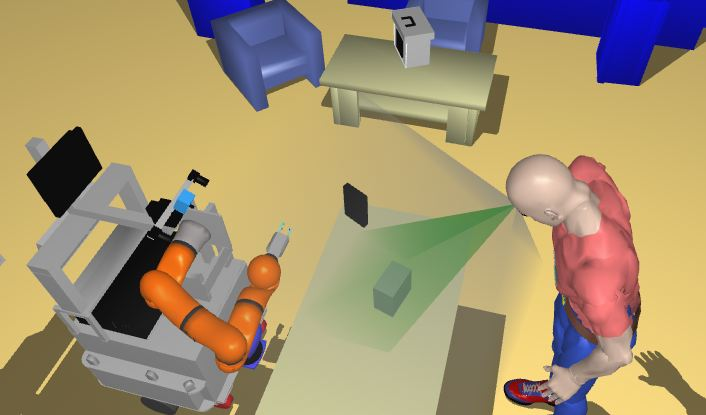
\includegraphics[width=0.4\linewidth]{spark/looks.jpg} 
    }
    \subfigure[]{
        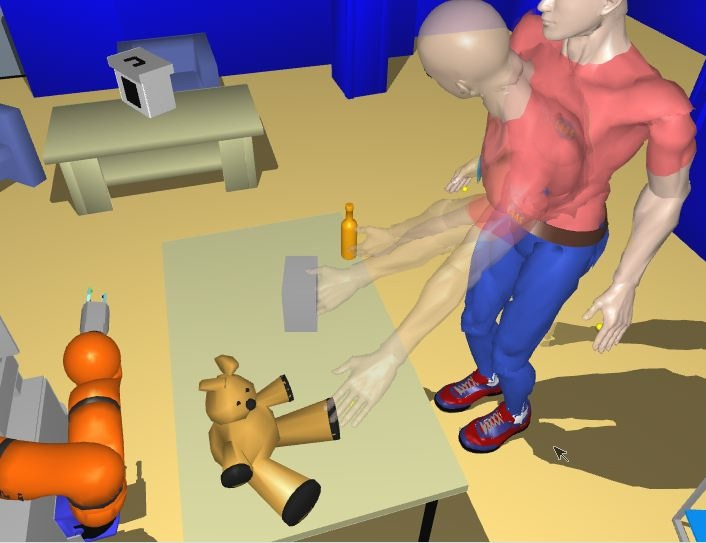
\includegraphics[width=0.35\linewidth]{spark/reach.jpg}
    }
    \caption{(a) Field of view (FOV) and the field of attention (FOA) of the
    human. (b) Different reaching postures for the human.}
    \label{fig::sparkRepresentations}
    \end{center}
\end{figure*} 


While the first three relations (\concept{sees}, \concept{looksAt} and
\concept{pointsAt}) are computed through a model based approach, the latter one
is based on the Generalized Inverse Kinematics with pseudo inverse
method~\cite{Nakamura90,Baerlocher04} to find a posture for the
agent where its end-effector is at the centre of the object within a given
tolerance.

Tables~\ref{facts|capabilites} summarises the predicates produced by SPARK
during the agent capabilities analysis phase.

\renewcommand{\concept}[1]{{\scriptsize \texttt{#1}}}
\begin{table}[h]
	\centering
		\begin{tabular}{p{2cm}lp{2cm}p{3.7cm}}
		\rowcolor{white}
		\textbf{Subject} & \textbf{Predicate} & \textbf{Object} & \emph{Notes} \\
		\hline
		 \concept{Agent}  & \concept{looksAt}  & \concept{SpatialThing} \\
		 \concept{Agent}  & \concept{sees}  &  \concept{SpatialThing}  &    \\ 
		 \concept{SpatialThing}  & \concept{isInFieldOfView}  &  \concept{xsd:boolean}  & via inference: \par \tiny \stmt{myself sees *} $\Leftrightarrow$ \stmt{* isInFieldOfView true} \\ 
		 \concept{Agent}  & \concept{pointsAt} $\equiv$ \concept{cyc:pointingToward}  & \concept{SpatialThing} \\ 
		 \concept{Agent}  & \concept{focusesOn}  &  \concept{SpatialThing}  &  via inference: \par \tiny \concept{looksAt} $\wedge$ \concept{pointsAt} $\Rightarrow$ \concept{focusesOn} \\
		\concept{Agent} & \concept{seesWithHeadMovement} &  \concept{SpatialThing} \\
		\concept{Agent} & \concept{reaches} &  \concept{Object} \\ 

	\end{tabular}

	\caption{List of facts describing the attentional state and the abilities
	of an agent. \concept{looksAt} is interpreted as an object \emph{being in
	the field of attention} of an agent. An object is seen if it is
	visible for the agent without moving the head (\ie, in \emph{field of
	view}).}

	\label{facts|capabilites}
\end{table}
\renewcommand{\concept}[1]{{\small \texttt{#1}}}

Table~\ref{facts|agentstate} lists the other symbolic facts that are
produced and maintained by SPARK related to the general state of the agent.

\renewcommand{\concept}[1]{{\scriptsize \texttt{#1}}}
\begin{table}[h]
	\centering
	\begin{tabular}{p{2cm}p{5cm}p{2cm}}
		\textbf{Subject} & \textbf{Predicate} & \textbf{Object} \\
		\hline
		\concept{Agent} & \concept{hasIn\{Left|Right\}Hand}  &  \concept{GraspableObject} \\ 
		\concept{Agent} & \concept{hasPosture}  &  \concept{Posture} \\
		\concept{Agent} & \concept{currentlyBodilyDoes}  &  \concept{Action}
	\end{tabular}

	\caption{List of statements describing the state of an agent in general.
	\concept{Posture} can be either \concept{standing} or \concept{sitting}.
	The \concept{currentlyBodilyDoes} predicate states the current action of
	the agent, be it intentional or not.}

	\label{facts|agentstate}
\end{table}
\renewcommand{\concept}[1]{{\small \texttt{#1}}}

%%%%%%%%%%%%%%%%%

\subsection{Symbolic task planning}
\label{sect|hatp}

Complex human robot interaction also requires reasoning about the actions the
agent can perform: How can they achieve a specific goal? What are the required
actions to achieve this goal? Which actions can be performed by each agent?
etc.

In the previous sections, we have seen how symbolic knowledge is produced and
stored from the real physical world. In this section, we present one possible
way to use these symbolic models of the environment and the interacting agents to
produce a plan of actions for a complex goal.

\begin{figure}
    \centering
    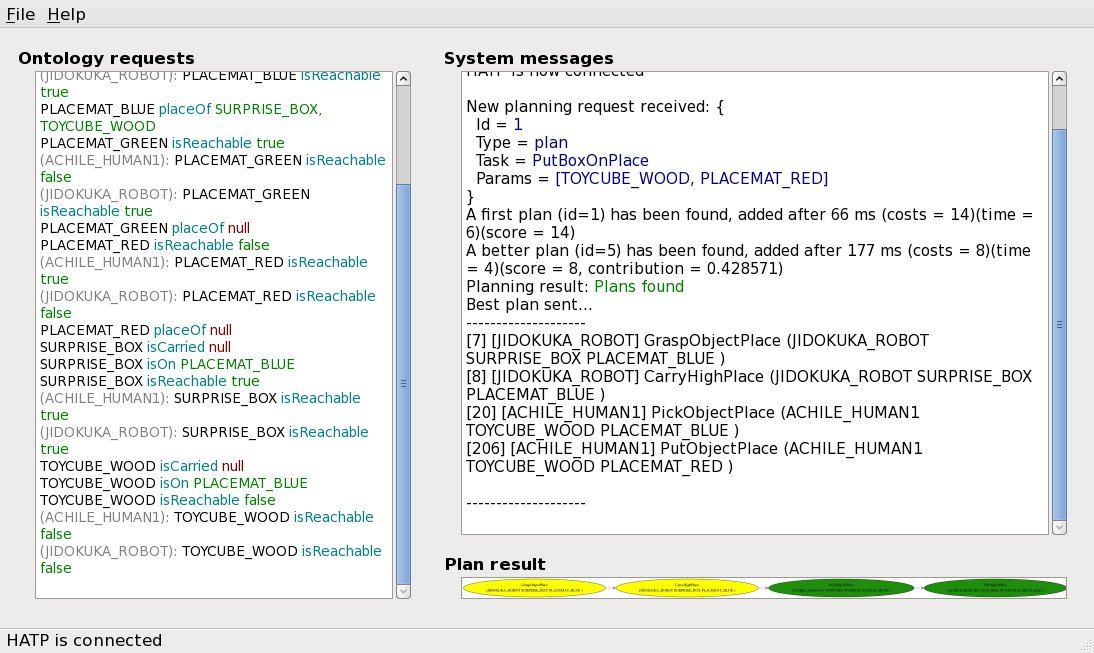
\includegraphics[width=0.9\columnwidth]{integration/hatp_console.jpg}
    \caption{Screenshot of the HATP console. On the left panel, we see the
    results of the requests to ORO, on the bottom right the resulting plan.}
    \label{fig|hatp_console}
\end{figure}

In order to devise how a given goal can be accomplished, the robot has to
elaborate a plan,\ie a set of actions to be achieved by the robot and its human
partners.  We use in our architecture the HATP planner~\cite{Alili2009} (for
Human Aware Task Planner, figure~\ref{fig|hatp_console}).  HATP is based on a
Hierarchical Task Network (HTN) refinement, which performs an iterative task
decomposition into sub-tasks until reaching atomic actions~\cite{Nau2003}.  The
planning domain defines a set of methods describing how to decompose a task and
can be seen as the procedural knowledge of the robot (note that this knowledge
in stored in the own resources of the planner, not in ORO).  HATP is able to
produce plans for the robot's actions as well as for the other agents. It can
be tuned by setting up different costs depending on the actions to apply and by
taking into account a set of constraints called \emph{social rules}. This
tuning aims at adapting the robot's behaviour according to the desired level of
cooperation of the robot.

\paragraph{Agents and action streams} The robot plans not only for itself but
also for the other agents. The planning domain of each agent is instantiated
from the agent-specific model in the ORO server. The resulting plan, called
``shared plan'' is a set of actions that form a stream for each agent involved
in the goal achievement.  Depending on the context, some ``shared plans''
contain causal relations between the agents. For example, the second agent
needs to wait for the success of the first agent's action to be able to start
its own action. When the plan is performed, causal links induce synchronisation
between agents.  Figure~\ref{plan_hatp1} illustrates a plan with two streams.

\begin{figure}[htbp]
  \centering
  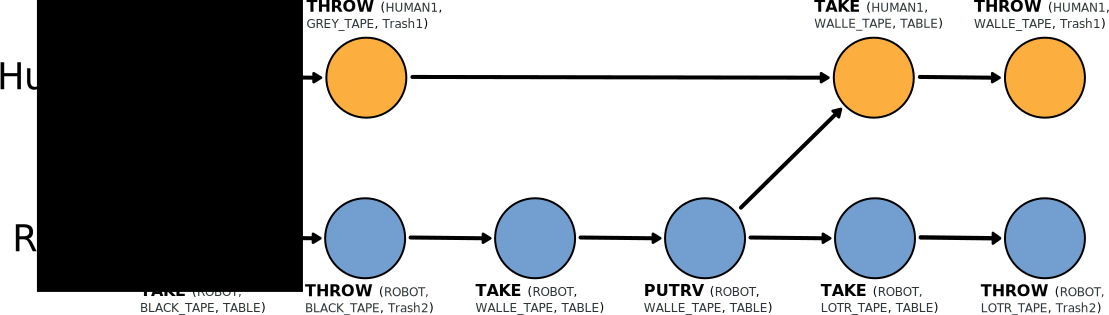
\includegraphics[width=0.8\columnwidth]{integration/hatp_plan1.pdf}
  \caption{A plan produced by HATP with 2 streams}
  \label{plan_hatp1}
\end{figure}

\paragraph{Action costs and social rules} A cost and a duration function is
associated to each action.  The duration function provides a duration interval
for the action achievement and is used, in one hand, to schedule the different
streams and, in the other hand, as an additional cost function.  In addition to
these costs, HATP also takes into account a set of social rules.  Social rules
are constraints aiming at leading the plan construction towards the best plan
according to some human preferences. The social rules we have defined so far
deal with:

\begin{itemize}

    \item undesirable state: to avoid a state in which the human could feel
    uncomfortable;

    \item undesirable sequence: to eliminate sequences of actions that can be
    misinterpreted by the human;

    \item effort balancing: to adjust the work effort of the agents;

    \item wasted time: used to avoid long delays between the actions of the
    human partner (figure~\ref{plan_hatp2});

    \item intricate links: to limit dependencies between the actions of two or
    more agents.

\end{itemize}

\begin{figure}[htbp]
  \centering
  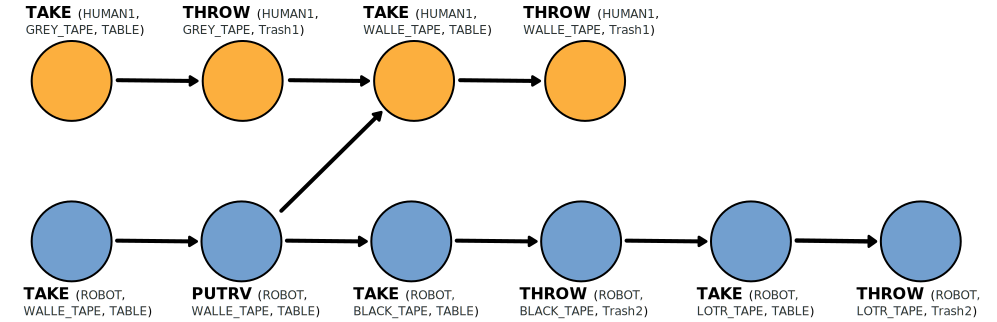
\includegraphics[width=0.8\columnwidth]{integration/hatp_plan2.pdf}
  \caption{Same plan with minimised wasted time.}
  \label{plan_hatp2}
\end{figure}

\paragraph{Several levels of cooperation} By tuning its costs and adapting its
social rules, HATP can be used to compute various alternative plans. These
plans can be categorised into several levels of cooperation

\begin{itemize}

    \item helping the human to achieve his goal by acting for him

    \item sharing concrete resources by handing some objects

    \item collaboration of the robot and the human by coordinating their
    actions towards a human-robot joint goal.

\end{itemize}


\subsection{Execution control}

Depending on experimental setups, the ORO server has been integrated with
several distinct execution controllers. We briefly present them here, with some
details regarding the integration knowledge base/controller.

\paragraph{CSLU Toolkit}
\label{sect|rad}

The CSLU Toolkit is a rapid application development framework developed at
Oregon University. It comprise of a suite of tools that enable exploration,
learning, and research into speech and human-computer interaction via a user
friendly graphical interface (figure~\ref{fig|rad}). The CSLU toolkit has been
employed in several experiments of the European FP7 CHRIS project (some are
presented at section~\ref{sect|casestudies}, others are presented
in~\cite{Lallee2010, Lallee2011}) to develop scripted verbal interactions with
robots.

\begin{figure}
    \centering
    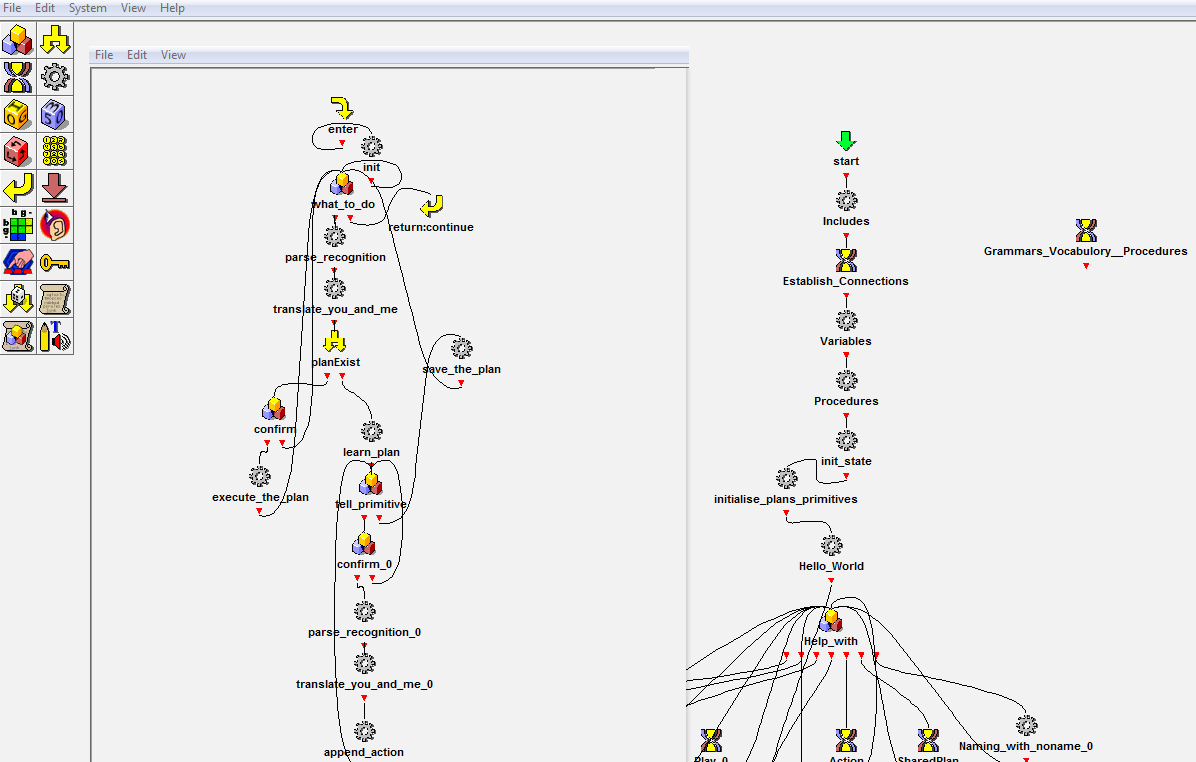
\includegraphics[width=0.8\columnwidth]{integration/rad.png}

    \caption{Example of graphical scripts produced with the CSLU Toolkit.
    Behaviours are programmed by building a network of connected ``boxes''.}

    \label{fig|rad}
\end{figure}

The CSLU Toolkit can be easily extended with the TCL scripting language, for
which bindings with the ORO server exist. This enable users to graphically
design interaction experiments that take advantage of the knowledge base and
its reasoning infrastructure to add and retrieve concepts.

\paragraph{CRAM}
\label{sect|cram}

{\sc Cram}~\cite{Beetz2010} (Cognitive Robotic Abstract Machine) is a
RPL-derived framework for rapid development of cognitive robot control programs
that is developed at the Intelligent Autonomous Systems at TU Munich.

The integration of ORO is seen as an extension to the robot's belief state that
not only contains abstract identifiers of the internal object representation
used in plans, but also the semantics and roles of objects in the scenario.

{\sc Cram} automatically updates the ORO server whenever an object enters or
leaves the field of view with a perception stack based on the \textsc{CoP}
framework~\cite{Klank2009}.

The \emph{Odd One Out} experiment (section~\ref{expe|odd_one_out}) relies on
{\sc Cram} for the robot control.

\paragraph{SHARY}

SHARY~\cite{Warnier2012} is a high level robot control system for cognitive
robot interacting with humans, based on the {\sc OpenPRS} environment (an
open-source implementation of PRS Procedural Reasoning
System~\cite{Ingrand1992}).

A full {\sc OpenPRS} interface with ORO has been developed, and request and
events mechanisms are heavily used by SHARY to monitor and react to changes in
the robot environment.

SHARY also produces symbolic facts that are added to the ORO server, including
the outcome of actions. This allows to partially expose the internal state of
the execution controller, and enhancing the introspective capabilities of the
system.

Finally SHARY can also directly interacts with situation assessment and
geometric layers (like the SPARK module), which indirectly influences the ORO
content. For instance, SHARY can create or delete position hypotheses for
currently unperceived objects, which in turn are converted into ({\it
de-facto}) hypothetical symbolic beliefs in the knowledge base.

Section~\ref{sect|expe3} presents an experiment that demonstrates the
integration between SHARY and ORO.

\paragraph{pyRobots} \label{sect|pyrobots} {\tt pyRobots} is not a real
execution controller: it comprise of a set of Python scripts that ease the
construction of complex scripted interaction. {\tt pyRobots} is based on
\emph{actions} (high-level tasks like {\tt goto}, {\tt pick} or {\tt
give}\footnote{The complete list is available online:
\url{http://www.openrobots.org/wiki/pyrobots}.}) that are combined into plans.

ORO server is integrated in {\tt pyRobots} via the ORO Python bindings
(presented at section~\ref{sect|python-bindings}). The action that is currently
performed, is maintained up-to-date in the server, and actions are free to
store or retrieve facts (for instance, the {\tt pick} task add the fact
\stmt{myself hasIn{Right|Left}Hand x}, \concept{x} being replaced by the ID of
the object that is taken.

Events can also be used by the application designer.


\subsection{Integration with natural language processors}

Figure~\ref{fig|dialog-integration} gives a functional overview of
components involved in the situated dialogue grounding.

\begin{figure}
    \centering
    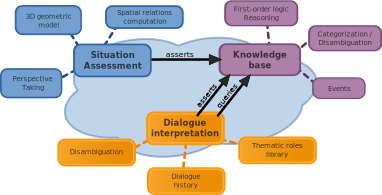
\includegraphics[width=0.7\columnwidth]{integration/dialog_integration.pdf}
    \caption{Schematic view of the integration of a natural language processor
    in the architecture}
    \label{fig|dialog-integration}
\end{figure}

Verbal interaction with a human is either initiated by the human or by the robot.

In case of human initiated dialogue, two main steps follow: understanding the
direct meaning of the sentence (what does the words mean?), and understanding
the intent of the sentence. The first step usually requires a large amount of
queries to the knowledge base to clarify and disambiguate the meaning of the
sentence ; the second step, depending on the intent (question, desire,
assertions), leads to either other queries (to answer a question) or new
assertions.

An interaction initiated by the robot usually follows an event triggered by the
controller (or possibly directly by the knowledge base). The dialogue that it
initiates then requires the same interaction capabilities with the knowledge
base that we mentioned in the previous paragraph.

Studying the integration of natural language grounding with a symbolic
knowledge base is one of the focus of the thesis, and the next chapter is
entirely dedicated to {\sc Dialogs}, a component for situated natural language
processing, and its integration with ORO.

%%%%%%%%%%%%%%%%%
%%%%%%%%%%%%%%%%%

\recap

This concludes the chapter~\ref{chapt|implementation-integration}. In this
chapter, we have first developed some technical and implementation-related
details, including the software architecture of the ORO server, examples of
integration with the Python and C++ API, and an overview of the visualisation
and debugging tools.

The chapter then focused on the actual integration of ORO server in existing
robotic architecture. We have first presented the software architecture of the
decisional layer of service robots at LAAS. We have introduced the SPARK module
for geometric reasoning and symbolic situation assessment and underline its
perspective taking capabilities.

We have finally presented briefly HATP, a symbolic task planner for human-robot
cooperative task planning that takes advantage of the ORO server for planning
initialisation, and mentioned four control environment that have been used with
ORO.

The next chapter is now dedicated to one specific application of the knowledge
base: situated natural language grounding.


